\documentclass[a4paper,12pt,notitlepage]{report}

\usepackage{float}
\usepackage{graphicx}
\usepackage[top=2.5cm, bottom=2.5cm, left=2.5cm, right=2.5cm]{geometry}
\usepackage{ifxetex}
\usepackage{fixltx2e}
\usepackage[super, square, comma, sort&compress]{natbib}
\usepackage{caption}
\usepackage{setspace}
\usepackage{subfig}
\usepackage{titlesec}
\usepackage{fancyhdr}
\usepackage{hyperref}
\usepackage{enumitem}
\usepackage{chngcntr}

\counterwithout{footnote}{chapter}

\ifxetex
    \usepackage{fontspec}
    \usepackage{xunicode}
    \setmainfont[Mapping=tex-text]{Segoe UI}
    \setmonofont[Ligatures={NoRequired,NoCommon,NoContextual}]{Consolas}
\else
    \usepackage[LGRx, T1]{fontenc}
    \usepackage[utf8x]{inputenc}
    \usepackage{textalpha}
    \usepackage{lmodern}
    \usepackage{microtype}
    \DisableLigatures{family=tt*}
\fi

\titleformat{\chapter}{\large\bfseries\selectfont}{\thechapter}{15pt}{}
\titlespacing*{\chapter}{0cm}{1cm}{0cm}[0cm]
\titleclass{\chapter}{straight}

\titleformat{\section}{\normalsize\bfseries\selectfont}{\thesection}{10pt}{}
\titleformat{\subsection}{\normalsize\bfseries\itshape\selectfont}{\thesubsection}{10pt}{}

\setcounter{tocdepth}{1}

\captionsetup[figure]{justification=justified, singlelinecheck=false, position=bottom, labelfont=bf, font=small}
\captionsetup[table]{justification=justified, singlelinecheck=false, position=bottom, labelfont=bf, font=small}
\DeclareSubrefFormat{subsimplebold}{\textbf{#2)}}
\captionsetup[subfigure]{format=hang, position=top, labelformat=simple, subrefformat=subsimplebold, captionskip=0pt, topadjust=0pt}
\renewcommand{\thesubfigure}{\Alph{subfigure}}
\DeclareCaptionLabelFormat{continued}{#1~#2 (cont.)}
\captionsetup[ContinuedFloat]{labelformat=continued}

\newcommand{\subfigureautorefname}{\figureautorefname}

\fancypagestyle{frontmatter}{
    \fancyhf{} % clear all header and footer fields
    \renewcommand{\headrulewidth}{0pt}
    \renewcommand{\footrulewidth}{0pt}
    \lhead{}
    \rhead{}
    \cfoot{-~\thepage~-}
    \pagenumbering{roman}
}
\fancypagestyle{main}{
    \fancyhf{} % clear all header and footer fields
    \renewcommand{\headrulewidth}{0.4pt}
    \renewcommand{\footrulewidth}{0pt}
    \lhead{\nouppercase\leftmark}
    \rhead{\nouppercase\rightmark}
    \cfoot{-~\thepage~-}
    \pagenumbering{arabic}
    \renewcommand{\chaptermark}[1]{\markboth{\thechapter.~##1}{}}
    \renewcommand{\sectionmark}[1]{\markright{\thesection.~##1}}
}

\newcommand{\myTitle}{{simpleSTORM: A self-calibrating single-molecule localization algorithm}}

\hypersetup{
    bookmarks=true,
    breaklinks=true,
    colorlinks=false,
    pdfborder={0 0 0},
    pdftitle=\myTitle
}

\renewcommand\bibname{References}
\renewcommand{\bibsection}{\chapter{\bibname}}

\setstretch{1.5}
\setlist{nosep, topsep=-\parskip}

\begin{document}
\bibliographystyle{unsrtnat_custom}
\begin{titlepage}
    \centering
    \vspace*{2cm}
    \Huge
    \myTitle

    \vspace{4cm}

    Hamprecht Lab, HCI/IWR\\
    Heidelberg, Germany

    \vspace{5cm}

    \the\year
    \thispagestyle{empty}
\end{titlepage}

\pagestyle{frontmatter}
\tableofcontents
\newpage

\parskip0.5cm
\parindent1cm
\titlespacing*{\section}{0cm}{0.75cm}{0cm}
\titlespacing*{\subsection}{0cm}{-0.5\parskip}{-\parskip}

\pagestyle{main}
\chapter{Introduction}
Conventional optical microscopy suffers from Abbe's resolution limit, which states that objects closer than about half the used wavelength can not be resolved. To be precise, the optical resolution limit is defined as the full width at half maximum (FWHM) of the objective's point spread function (PSF), which can be expressed as $\frac{\lambda}{2 \cdot \mathit{NA}}$ within the focus plane, with λ being the wavelength and NA the numerical aperture of the objective used, typically about 1-1.5. Several techniques have been developed to overcome this limitation. The most widely used include STORM\citep{pmid16896339} (stochastic optical reconstruction microscopy), dSTORM\citep{pmid18646237} (direct STORM) and PALM\citep{pmid16902090} (photoactivated localization microscopy). All of these are commonly known as single-molecule localization microscopy and are based on the common principle of taking multiple images per sample, with only a small subset of fluorophores being excited at each frame. The objective's PSF can then be fitted to the individual intensity distributions, yielding a precise molecule localization with a resolution of about 20 nm\citep{pmid18646237}.

Although numerous software applications for single-molecule localization have been published\citep{pmid23132113, pmid20431545, pmid22522657}, these usually offer a plethora of configuration possibilites, raising the entry threshold for the localization microscopy novice. simpleSTORM aims to provide good localization results with virtually no user input while still allowing manual fine-tuning of the necessary parameters.


\chapter{Installation}

\section{Binary packages}
Look in README.md for up-to-date infromation of binary packages.

\section{Compiling from source}
\subsection{Dependencies}
\begin{itemize}
    \item A recent C++ compiler with C++11 support (Any GCC version >= 4.7 will do the job)
    \item VIGRA and its dependencies
    \item libfftw in both single and double precision
    \item librudeconfig
    \item libhdf5 (optional)
    \item Qt 4 >= 4.6
    \item CMake >= 2.8
\end{itemize}

\subsection{Compiling}
Compilation follows the standard procedures. After running CMake, specifying the paths to the dependencies manually if required, simpleSTORM can be compiled, e.g. by running \texttt{make} on GNU/Linux, MacOSX, or Windows when using MinGW. Installer packages on Windows and MacOSX can be built by issuing the \texttt{make package} command. When using MinGW on Windows, be sure to use a threading-capable version\footnote{\url{http://sourceforge.net/projects/mingwbuilds/}}. When using Clang on MacOSX, the Clang standard C++ library has to be used for C++11 suppport. This can be accomplished by adding \texttt{-stdlib=libc++} to \texttt{CMAKE\_CXX\_FLAGS} in CMake.

\chapter{GUI manual}
\section{Input}
\begin{figure}[ht]
    \subfloat[]{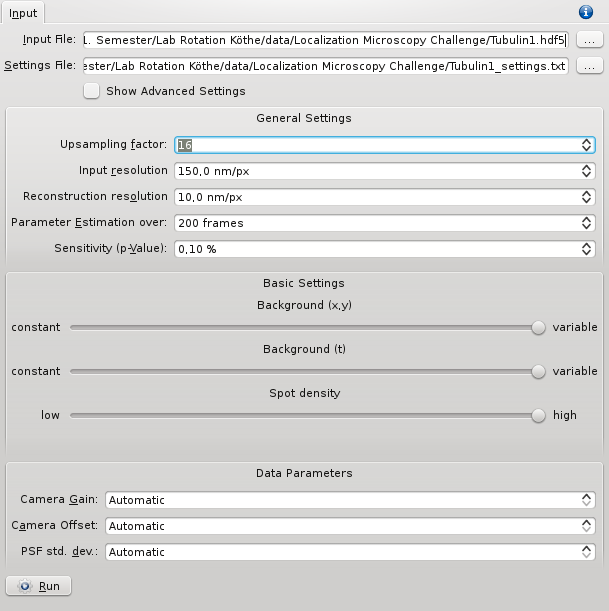
\includegraphics[width=0.49\textwidth]{images/input_simple.png}\label{fig:input_simple}}\hfill
    \subfloat[]{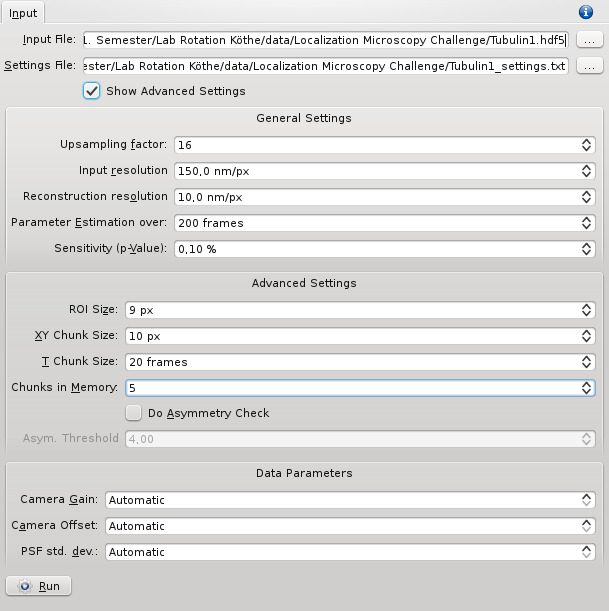
\includegraphics[width=0.49\textwidth]{images/input_advanced.png}\label{fig:input_advanced}}
    \caption[]{The input window of simpleSTORM. \subref*{fig:input_simple} The basic view for users not familiar with the algorithm. \subref*{fig:input_advanced} The advanced view for expert users.}
    \label{fig:input}
\end{figure}

simpleSTORM can process TIFF, SIF and HDF5 files, the path to the input file can be entered manually, selected by clicking on the button next to the ``Input File'' field or the file can simply be dragged into it. If the file is valid, the rest of the buttons and fields will be enabled. Additionally, a settings file can be specified where the selected and estimated parameters will be saved to. If the specified settings file already exists, its contents will be used to preset the current values.

Additional parameters that can be specified are:
\begin{description}
    \item[Upsampling Factor] Interpolation factor for the last stage of the algorithm. A higher value improves precision, but is computationally more intensive.
    \item[Input resolution] Resolution of the input images in nm/px. Used to determine the resolution of the reconstructed image.
    \item[Reconstruction resolution] The desired resolution of the reconstructed image in nm/px. Note that this can not be lower than $\mathrm{\frac{upsampling\ factor}{input\ resolution}}$.
    \item[Parameter estimation over] Estimation of camera gain and offset as well as the PSF width will be performed over only the first N frames, where N is the value in this input field.
    \item[Sensitivity (p-value)] The threshold for mask computation. A higher value will result in more detections, but also more false positives (i.e. higher recall with lower precision), while a lower value will increase the precision but decrease recall.
    \item[Background (x,y) (simple mode only)] Background variability in space. This influences the chunk size in X and Y. A higher setting will result in smaller chunks.
    \item[Background (t) (simple mode only)] Background variability in time. This influences the chunk size in t. A higher setting will result in smaller chunks
    \item[Spot density (simple mode only)] Density of fluorescence spots. A higher value will increase the asymmetry threshold, allowing merged spots to be detected, but also potentially increasing the false positive rate, while a lower value will result in a lower asymmetry threshold, removing asymmetrical spots.
    \item[ROI Size (advanced mode only)] Size of the ROI used for upsampling in pixels. Also influences ROI size for PSF estimation.
    \item[XY Chunk Size (advanced mode only)] Size of chunks in space in pixels. Lower values are suitable for highly dynamic background.
    \item[T Chunk Size (advanced mode only)] Size of chunks in time in pixels. Lower values are suitable for highly dynamic background.
    \item[Chunks in Memory (advanced mode only)] Number of chunks to keep in memory simultaneously. A higher value will improve background interpolation at the cost of increased memory consumption.
    \item[Do Asymmetry Check (advanced mode only)] Whether to filter false positives by asymmetry.
    \item[Asym. Threshold (advanced mode only)] Threshold of the Hessian eigenvalues ratio for asymmetry detection. A higher value will allow for asymmetrical spots to be detected.
    \item[Camera Gain] Camera gain if known. Input the value "0" to trigger automatic estimation ("self-calibration"). Other vallues are interpreted as user supplied settings. If a "settings file" exists for the given dataset, a suitable value is read from that file.
    \item[Camera Offset] Camera offset if known. Input the value "0" to trigger automatic estimation ("self-calibration"). Other vallues are interpreted as user supplied settings. If a "settings file" exists for the given dataset, a suitable value is read from that file.
    \item[PSF std. dev.] Standard deviation of the point spread function. Input the value "0" to trigger automatic estimation ("self-calibration"). Other vallues are interpreted as user supplied settings. If a "settings file" exists for the given dataset, a suitable value is read from that file.
\end{description}

\section{Results}
\begin{figure}[ht]
    \subfloat[]{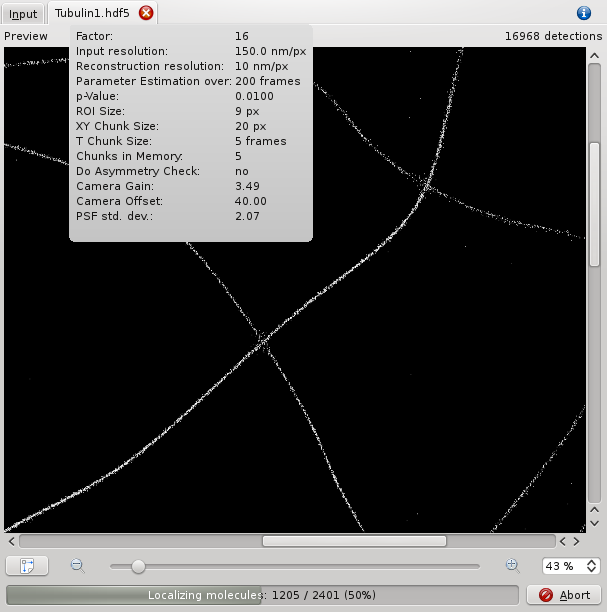
\includegraphics[width=0.49\textwidth]{images/result_progress.png}\label{fig:result_progress}}\hfill
    \subfloat[]{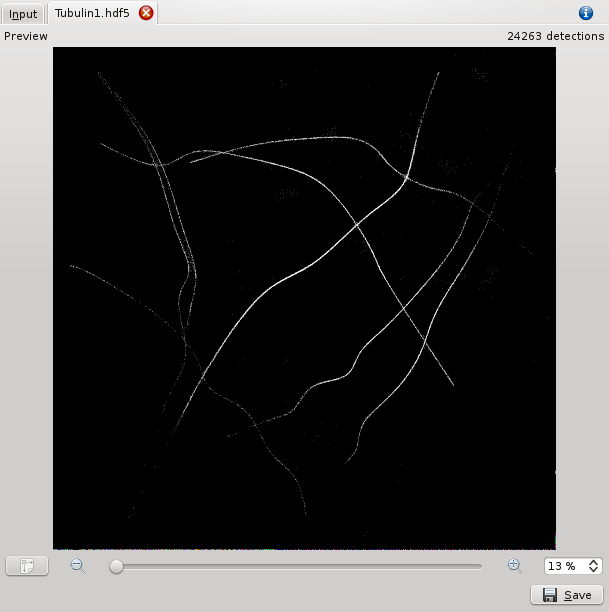
\includegraphics[width=0.49\textwidth]{images/result_finished.png}\label{fig:result_finished}}
    \caption[]{After supplying suitable input and hitting the run button, a new tab with the result will be opened. \subref*{fig:result_progress} While computation is in progress, a progress bar will be displayed. \subref*{fig:result_finished} The result can be saved after the computation is finished.}
    \label{fig:result}
\end{figure}
After hitting the Run button, a new tab showing the progress and a live preview will be opened. Several jobs can run simultaneously, the parameters of a job can be shown by hovering with the mouse over the respective tab (\autoref{fig:result_progress}). After the computation is completed (\autoref{fig:result_finished}), the results can be saved as a text file with the localizations, a high-resolution image (32-bit TIFF, can be opened with ImageJ), or both.

\chapter{Commandline Interface (CLI) manual}
\section{Synopsis}
\textbf{storm [OPTIONS] input-file}
\section{Description}
\begin{description}[format=\bfseries\ttfamily]
    \item[-?, --help] Print help message and exit.
    \item[-v, --verbose] Print debug messages during localization.
    \item[-V, --version] Print version information and exit.
    \item[-g factor, --factor=factor] The upsampling factor. Default: 8.
    \item[-P frames, --cam-param-frames=frames] The number of frames to perform parameter estimation over. Default: 200.
    \item[-c file, --coordsfile=file] The path to the output localizations file. Default: path to input file with .txt extension.
    \item[-p size, --pixelsize=size] Pixel size in nanometers. Default: 1 (i.e. the localizations will be in pixel coordinates)
    \item[-s file, --settings=file] Path to settings file. Default: input-file\_settings.txt . Parameters used for localization as well as estimated parameters will be stored here and loaded upon re-running simpleSTORM. Parameters without command-line options can be changed here, as well.
    \item[-m size, --roi-len=size] ROI size in pixels. Default: 9
    \item[-a thresh, --asymmetry-threshold=thresh] Threshold for asymmetry-based false positive filtering. Default: 4
\end{description}

\chapter{Algorithm}
The localization algorithm is subdivided into four stages. In stage 1, the camera gain and offset are being estimated using difference-based noise modeling in the time dimension\citep{journals/pami/HwangKK12}. After constructing a mean projection over a subset of frames, the algorithm attempts to select pixels over the entire value range, for which the µ\textsuperscript{(1)} skellam parameter is computed. A linear function is then fitted to the µ\textsuperscript{(1)}/mean value plot, whose slope and root are assumed to be the camera gain and offset, respectively. To account for pixels containing signal in a subset of frames, which generally significantly deviate from the linear relationship between the mean value and µ\textsuperscript{(1)}, fitting is only performed over the most compact subset of data points\citep{jstor1270566}.

A common pre-processing step is applied to stages 2-4, consisting of transformation of the image data to a Poisson distribution using the parameters obtained in stage 1, transformation of the Poisson distributed image into a unit-variance Gaussian using the Anscombe transform\citep{jstor2332343}, and local background subtraction. For the background estimation, the image stack is subdivided into 3-dimensional chunks, for each chunk the median, which for a Gaussian distribution is identical to the mean, but better suited here due to its resistance to outliers such as pixels with signal, is computed. The low-resolution median image is interpolated to the original resolution using a cubic B-spline and the interpolated image subtracted from the original. To conserve memory, the image stack is processed incrementally, with at most 5 (in the default configuration) t-chunks kept in memory. This strategy results in the preprocessing having to be repeated for each of the three stages where it is applied.

The camera gain estimated in stage 1 is further refined in stage 2 by an iterative algorithm. As an incorrect gain estimate results in a non-Poisson distribution and thus directly affects the variance of the Gaussian distribution after the Anscombe transform, a 1D Gaussian PDF is fitted to the histograms of a subset of frames after pre-processing, the gain adjusted (using the estimate from stage 1 as a starting value) until the mean variance converges to 1. The obtained gain value is used in pre-processing for the subsequent stages.

A good PSF estimate is key to optimal localization results. simpleSTORM assumes the PSF to be a 2D-Gaussian with equal variance in X- and Y-direction. In stage 3 a subset of frames is processed, for each frame several randomly chosen local maxima above a dynamically computed threshold are chosen and the Fourier transform of a region (subsequently referred to as ROI, region of interest) around each maximum is computed. As applying the Fourier transform to a Gaussian signal in the time or spatial domain results in a normally distributed signal in the frequency domain with the variances being inversely proportional to each other (the exact formula is shown in \autoref{eqn:freq_spatial_sd}, where N is the ROI width in pixels, σ\textsubscript{s} the standard deviation of the Gaussian in spatial domain and σ\textsubscript{f} the standard deviation of the Gaussian in frequency domain), a 2D Gaussian PDF is fitted to the mean magnitude image obtained from all frequency spectra and its variance used to compute the PSF variance in the spatial domain.
\begin{equation}
    \sigma_s = \frac{N}{2 \cdot \pi \cdot \sigma_f}
    \label{eqn:freq_spatial_sd}
\end{equation}

Fluorophore localization happens in stage 4. The pre-processed image is convolved with a Gaussian filter using the variance estimated in stage 3, as this so-called matched filtering results in an optimal signal-to-noise ratio (SNR). To roughly localize the signal the filtered image is thresholded with a user-supplied p-value under the assumption of a zero-mean, unit variance Gaussian distribution, the threshold being corrected for the filtering. Regions around local maxima with an intensity above the threshold are interpolated using a cubic B-spline and a user-defined interpolation factor, the local maximum of the upsampled ROI is assumed to correspond to the fluorophore coordinate. To reduce false positives a filtering based on spot asymmetry, computed via the eigenvalues ratio of the Hessian matrix at the maximum, can be applied.

\bibliography{literature}

\end{document}
